\documentclass[handout]{beamer}
\usepackage[T1]{fontenc}
\usepackage[utf8]{inputenc}
\usepackage{lmodern}
\usepackage[italian]{babel}

\title{Le reti e la sicurezza informatica}
\author{Mattia Cozzi\newline\href{mailto:cozzimattia@gmail.com}{\texttt{cozzimattia@gmail.com}}}
\date{a.s.~2023/2024}


%\documentclass[handout]{beamer}     %usare questa classe per generare l'handout

%\usepackage{pdfpages}   %per mostrare più quadri nella stessa pagina
%\pgfpagesuselayout{4 on 1}[a4paper,border shrink=5mm,landscape]


\usetheme{Singapore}
%\useoutertheme[left]{sidebar} %elementi intorno alle diapositive
\setbeamercovered{dynamic} %modifica l'aspetto del testo grigetto delle diapositive future. Argomenti: invisible/transparent/dynamic


%COLORE PRINCIPALE
\definecolor{verde}{RGB}{2, 194, 117} % UBC Blue (primary)
\setbeamercolor{structure}{fg=verde} % itemize, enumerate, etc
\setbeamercolor{alerted text}{fg=verde}


\usecolortheme{orchid}

\usepackage{tikz}

\begin{document}

\begin{frame}
  \titlepage
\end{frame}


\begin{frame}
\frametitle{Contenuti}
\tableofcontents
\end{frame}



\section{Classificazioni}


\begin{frame}
\frametitle{Collegamento}
I computer vengono collegati tra loro per:
\begin{itemize}
  \item comunicare tra loro;\pause
  \item condividere risorse:\pause
  \begin{itemize}
    \item hardware (stampanti);\pause
    \item files (su dischi fissi condivisi);\pause
    \item programmi o interi sistemi operativi;\pause
  \end{itemize}
\end{itemize}

~

Il collegamento avviene tramite un componente hardware chiamato \alert{scheda di rete}.
\end{frame}


\begin{frame}
\frametitle{Dimensione delle reti}
Possiamo classificare le reti in base alla loro \alert<1>{dimensione}:\pause
\begin{description}
  \item[(W)LAN] (Local Area Network), terminali connessi nello stesso luogo (casa, ufficio);\pause
  \item[MAN] (Metropolitan Area Network), terminali in un'area urbana o comuni limitrofi;\pause
  \item[WAN] (Wide Area Network), terminali in un'intera nazione;\pause
  \item[GAN] (Global Area Network), terminali in tutti i continenti.
\end{description}\pause

~

Ogni terminale è identificato da un numero, l'indirizzo MAC (Media Access Control), univoco.
\end{frame}


\begin{frame}
\frametitle{Modello client/server e peer to peer}
Come avviene la condivisione di risorse?\pause

~

Dividiamo le reti in due classi:
\begin{description}
  \item[client/server] alcuni computer (server o host) mettono a disposizione risorse, altri (client) le utilizzano;\pause
  \item[peer to peer] tutti i computer condividono le loro risorse e tutti possono utilizzarle.\pause
\end{description}

~

Nel modello peer to peer ogni computer è sia server sia client.
\end{frame}

\begin{frame}
\frametitle{Schema del modello client-server}
\begin{figure}
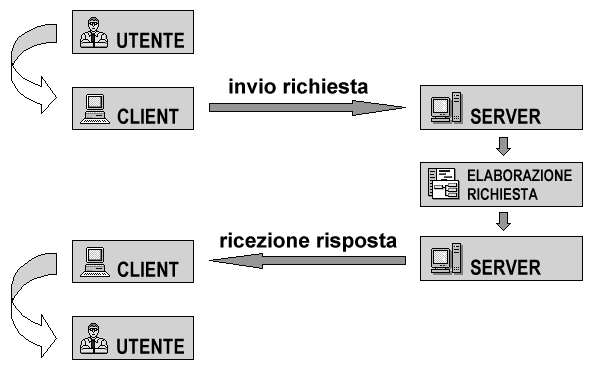
\includegraphics[width=.7\columnwidth]{screenshots/clientserver.png}
\end{figure}
\end{frame}


\section{Topologia}


\begin{frame}
\frametitle{Topologia delle reti}
\begin{figure}
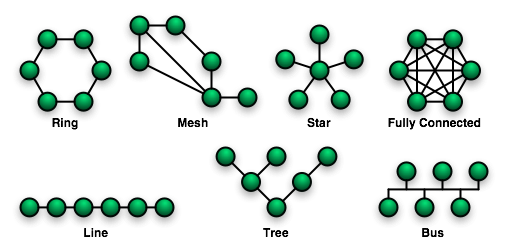
\includegraphics[width=.7\columnwidth]{screenshots/reti.png}
\end{figure}
\end{frame}



\section{Internet}


\begin{frame}
\frametitle{Scambio di informazioni}

  

\end{frame}




\begin{frame}
\frametitle{Internet}

  
\end{frame}



\begin{frame}
\frametitle{Navigare in rete}

  

\end{frame}




\begin{frame}
\frametitle{Il web}

  

\end{frame}



\begin{frame}
\frametitle{Il protocollo HTML}

  

\end{frame}


\begin{frame}
\frametitle{Protocollo TCP-IP}

  

\end{frame}


\begin{frame}
\frametitle{Browser}


\end{frame}



\begin{frame}
\frametitle{Motori di ricerca}

  

\end{frame}


\begin{frame}
\frametitle{La posta elettronica}

  

\end{frame}


\begin{frame}
\frametitle{Intranet ed Extranet}

  

\end{frame}

\begin{frame}
\frametitle{Social media}

  

\end{frame}


\section{Sicurezza}



\begin{frame}
\frametitle{Privacy}

  

\end{frame}

\begin{frame}
\frametitle{Cookies}

  

\end{frame}


\begin{frame}
\frametitle{Tutela dei dati}

  

\end{frame}





\begin{frame}
\frametitle{Firewall}

  

\end{frame}





\begin{frame}
\frametitle{Antivirus}

  

\end{frame}




\begin{frame}
\frametitle{Phishing}

  

\end{frame}






\begin{frame}
\frametitle{Malware}

  

\end{frame}







\begin{frame}
\frametitle{Spam}



\end{frame}





\begin{frame}
\frametitle{Uso consapevole dei social media}

  

\end{frame}



\end{document}
